% !TEX program = xelatex
\documentclass[12pt,a4paper,oneside]{report}
\newcommand{\University}{TRƯỜNG ĐẠI HỌC [ĐIỀN TÊN TRƯỜNG]}
\newcommand{\Faculty}{KHOA [ĐIỀN TÊN KHOA]}
\newcommand{\CourseName}{PBL5 -- HỆ THỐNG MÁY TÍNH}
\newcommand{\ReportTitle}{BÁO CÁO TIẾN ĐỘ DỰ ÁN\\NHẬN DẠNG KỸ THUẬT CẦU LÔNG TỪ CHUỖI KHỚP CƠ THỂ}
\newcommand{\StudentName}{Khắc Bình}
\newcommand{\StudentID}{[ĐIỀN MSSV]}
\newcommand{\ClassName}{[ĐIỀN LỚP]}
\newcommand{\Supervisor}{[ĐIỀN GIẢNG VIÊN HƯỚNG DẪN]}
\usepackage[a4paper,top=2.4cm,bottom=2.4cm,left=3cm,right=2cm]{geometry}
\usepackage{fontspec}
\IfFontExistsTF{Times New Roman}{\setmainfont{Times New Roman}}{\setmainfont{TeX Gyre Termes}}
\usepackage{amsmath,amssymb,graphicx,booktabs,longtable,tabularx,array,float}
\usepackage{caption,subcaption,enumitem,setspace,xcolor,hyperref,tikz,titlesec}
\usetikzlibrary{arrows.meta,positioning,shapes.geometric}
% Cỡ chữ chuẩn cho toàn bộ nội dung chính: 14 pt, giãn dòng 18 pt.
\AtBeginDocument{\fontsize{14pt}{18pt}\selectfont}
\setstretch{1.3}
\setlength{\parindent}{1.2cm}
\setlength{\parskip}{0.25em}
\setcounter{tocdepth}{2}

% Hệ thống cấp chữ thống nhất.
\titleformat{\chapter}[display]
  {\bfseries\fontsize{18pt}{22pt}\selectfont}
  {\chaptername\ \thechapter}{0.45em}{\MakeUppercase}
\titlespacing*{\chapter}{0pt}{-12pt}{18pt}
\titleformat{\section}
  {\bfseries\fontsize{16pt}{20pt}\selectfont}
  {\thesection}{0.65em}{}
\titlespacing*{\section}{0pt}{16pt}{8pt}
\titleformat{\subsection}
  {\bfseries\fontsize{14pt}{18pt}\selectfont}
  {\thesubsection}{0.65em}{}
\titlespacing*{\subsection}{0pt}{12pt}{6pt}
\renewcommand{\contentsname}{MỤC LỤC}
\renewcommand{\listfigurename}{DANH MỤC HÌNH}
\renewcommand{\listtablename}{DANH MỤC BẢNG}
\renewcommand{\chaptername}{Chương}
\renewcommand{\figurename}{Hình}
\renewcommand{\tablename}{Bảng}
\renewcommand{\bibname}{TÀI LIỆU THAM KHẢO}
\DeclareCaptionFont{fourteenpt}{\fontsize{14pt}{18pt}\selectfont}
\captionsetup{font=fourteenpt,labelfont=bf,labelsep=period}
\hypersetup{colorlinks=true,linkcolor=black,citecolor=black,urlcolor=blue}
\newcolumntype{Y}{>{\raggedright\arraybackslash}X}
\newcommand{\code}[1]{\texttt{\detokenize{#1}}}
\newcommand{\vect}[1]{\boldsymbol{#1}}
\newcommand{\done}{\textcolor{green!50!black}{\textbf{Hoàn thành}}}
\newcommand{\doing}{\textcolor{orange!80!black}{\textbf{Đang mở rộng}}}

\begin{document}
\begin{titlepage}
\begin{center}
{\bfseries\fontsize{14pt}{18pt}\selectfont \University\par}
\vspace{0.25cm}
{\bfseries\fontsize{14pt}{18pt}\selectfont \Faculty\par}
\vspace{2cm}
{\bfseries\fontsize{18pt}{22pt}\selectfont \CourseName\par}
\vspace{1.2cm}
{\bfseries\fontsize{19pt}{25pt}\selectfont \ReportTitle\par}
\vspace{1cm}
{\large YOLO26 Pose -- MotionBERT -- ST-GCN\par}
\vfill
\begin{tabular}{>{\bfseries}p{5cm}p{8cm}}
Sinh viên thực hiện: & \StudentName\\
Mã số sinh viên: & \StudentID\\
Lớp: & \ClassName\\
Giảng viên hướng dẫn: & \Supervisor\\
\end{tabular}
\vfill
{\bfseries Đà Nẵng, ngày 18 tháng 11 năm 2026}
\end{center}
\end{titlepage}

\pagenumbering{roman}
\chapter*{TÓM TẮT TIẾN ĐỘ}
\addcontentsline{toc}{chapter}{TÓM TẮT TIẾN ĐỘ}

Dự án xây dựng hệ thống nhận dạng 18 kỹ thuật cầu lông từ clip ngắn của tập VideoBadminton. Pipeline hiện tại gồm YOLO26s Pose trích xuất 17 điểm khớp COCO 2D, MotionBERT nâng chuỗi khớp lên skeleton Human3.6M 3D, và ST-GCN học quan hệ không gian--thời gian để phân loại kỹ thuật.

Đến thời điểm báo cáo, các bước kiểm tra và chia dữ liệu, trích xuất pose 2D, suy luận pose 3D, huấn luyện ST-GCN 2D, huấn luyện ST-GCN 3D và bốn thí nghiệm ablation đã hoàn thành. Tập dữ liệu cục bộ có 7.821 clip thuộc 18 lớp. YOLO26 Pose xử lý thành công 7.818 clip, đạt 99,96\%. ST-GCN V2 dùng pose 2D đạt test accuracy 60,17\% và Macro F1 0,3882. Phiên bản dùng MotionBERT 3D đạt test accuracy 63,90\% và Macro F1 0,4209.

Kho mã đã được tổ chức thành các mô-đun trong \code{src/}, script trong \code{scripts/}, chương trình huấn luyện trong \code{experiments/} và notebook trong \code{notebooks/}. Năm smoke test về cấu trúc, đồng bộ notebook và forward pass đều vượt qua.

\noindent\textbf{Từ khóa:} cầu lông, nhận dạng hành động, YOLO26 Pose, MotionBERT, ST-GCN, skeleton 3D.

\tableofcontents
\listoffigures
\listoftables
\clearpage
\pagenumbering{arabic}

\chapter{TỔNG QUAN DỰ ÁN}
\section{Bài toán và mục tiêu}

Đầu vào là một clip cầu lông đã được cắt theo một động tác; đầu ra là một trong 18 nhãn kỹ thuật:
\begin{equation}
f:\mathbb{R}^{T\times H\times W\times 3}\rightarrow\{0,1,\ldots,17\}.
\end{equation}
Dự án chuyển video thành chuỗi khớp để giảm ảnh hưởng của nền sân và tập trung vào chuyển động cơ thể.

Các mục tiêu chính gồm:
\begin{itemize}
\item kiểm tra dữ liệu và tạo manifest;
\item chia train, validation và test theo phiên quay;
\item trích xuất skeleton 2D bằng YOLO26s Pose;
\item nâng skeleton 2D thành 3D bằng MotionBERT;
\item xây dựng ST-GCN cho COCO và Human3.6M;
\item đánh giá bằng accuracy, Macro F1, weighted F1 và ma trận nhầm lẫn;
\item thực hiện ablation và tổ chức mã nguồn có khả năng tái lập.
\end{itemize}

\section{Phạm vi}

Hệ thống phân loại clip đã cắt sẵn, chưa phát hiện ranh giới động tác trong video dài. YOLO26 Pose và MotionBERT dùng trọng số tiền huấn luyện; ST-GCN được huấn luyện cho 18 lớp. Hệ thống chưa dùng trực tiếp ảnh RGB, vợt, shuttlecock, court homography hoặc âm thanh.

\chapter{DỮ LIỆU VÀ TIỀN XỬ LÝ}
\section{Dữ liệu và cách chia}

Dữ liệu lấy từ VideoBadminton \cite{videobadminton}. Phiên bản cục bộ sau kiểm tra có 7.821 clip, 18 lớp và 80 phiên quay. Các kiểm tra gồm file không rỗng, khoảng frame hợp lệ, mã người chơi hợp lệ, mã lớp khớp thư mục và video có thể đọc.

Dữ liệu được chia theo \code{source_id} tạo từ ngày và thời gian phiên quay. Toàn bộ clip của cùng một phiên chỉ thuộc một split, nhờ đó giảm nguy cơ model ghi nhớ bối cảnh phiên quay.

\begin{table}[H]
\centering
\caption{Quy mô các tập dữ liệu}
\begin{tabular}{lrrrr}
\toprule
\textbf{Split} & \textbf{Clip} & \textbf{Tỷ lệ} & \textbf{Phiên} & \textbf{Frame TB}\\
\midrule
Train & 5.465 & 69,87\% & 56 & 34,02\\
Validation & 1.176 & 15,04\% & 12 & 34,63\\
Test & 1.180 & 15,09\% & 12 & 33,65\\
\midrule
Tổng & 7.821 & 100\% & 80 & 34,07\\
\bottomrule
\end{tabular}
\end{table}

\section{Phân bố lớp}

\begin{longtable}{p{5.2cm}rrr}
\caption{Số mẫu theo lớp và split}\\
\toprule
\textbf{Lớp} & \textbf{Train} & \textbf{Validation} & \textbf{Test}\\
\midrule
\endfirsthead
\toprule
\textbf{Lớp} & \textbf{Train} & \textbf{Validation} & \textbf{Test}\\
\midrule
\endhead
Short Serve & 620 & 129 & 132\\
Cross Court Flight & 111 & 20 & 35\\
Lift & 529 & 102 & 127\\
Tap Smash & 73 & 15 & 21\\
Block & 215 & 42 & 59\\
Drop Shot & 560 & 130 & 122\\
Push Shot & 300 & 50 & 51\\
Transitional Slice & 79 & 26 & 18\\
Cut & 406 & 78 & 101\\
Rush Shot & 102 & 5 & 6\\
Defensive Clear & 78 & 22 & 9\\
Defensive Drive & 108 & 3 & 0\\
Clear & 644 & 158 & 143\\
Long Serve & 680 & 161 & 150\\
Smash & 576 & 127 & 119\\
Flat Shot & 226 & 71 & 30\\
Rear Court Flat Drive & 71 & 26 & 24\\
Short Flat Shot & 87 & 11 & 33\\
\midrule
Tổng & 5.465 & 1.176 & 1.180\\
\bottomrule
\end{longtable}

Dữ liệu mất cân bằng: Long Serve có 680 mẫu train trong khi Rear Court Flat Drive có 71. Defensive Drive không có mẫu test do ưu tiên group split. Do đó accuracy phải được đọc cùng Macro F1 và chỉ số từng lớp.

\chapter{PIPELINE ĐÃ XÂY DỰNG}
\section{Kiến trúc tổng thể}

\begin{figure}[H]
\centering
\resizebox{\textwidth}{!}{
\begin{tikzpicture}[
node distance=0.6cm,
block/.style={rectangle,rounded corners,draw=black,fill=blue!7,minimum width=2.6cm,minimum height=1cm,align=center},
arrow/.style={-{Latex[length=2.4mm]},thick}
]
\node[block] (a) {Video clip};
\node[block,right=of a] (b) {YOLO26 Pose\\COCO-17 2D};
\node[block,right=of b] (c) {COCO sang H36M\\Nội suy};
\node[block,right=of c] (d) {MotionBERT\\H36M-17 3D};
\node[block,right=of d] (e) {Chuẩn hóa\\Motion};
\node[block,right=of e] (f) {ST-GCN V2\\Attention};
\node[block,right=of f] (g) {18 lớp};
\draw[arrow] (a)--(b);
\draw[arrow] (b)--(c);
\draw[arrow] (c)--(d);
\draw[arrow] (d)--(e);
\draw[arrow] (e)--(f);
\draw[arrow] (f)--(g);
\end{tikzpicture}}
\caption{Pipeline hiện tại của dự án}
\end{figure}


\section{YOLO26 Pose và biểu diễn 2D}

Mỗi frame được suy luận ở kích thước 640 pixel với ngưỡng người 0,25 và ngưỡng keypoint 0,25. Nếu phát hiện nhiều hơn hai người, hệ thống giữ hai bounding box lớn nhất và sắp xếp theo tọa độ dọc thành slot Top và Bottom.

Đầu ra của một clip:
\begin{align}
\vect{J}^{2D}&\in\mathbb{R}^{T\times2\times17\times2},\\
\vect{S}^{2D}&\in[0,1]^{T\times2\times17}.
\end{align}
Keypoint dưới ngưỡng được đặt tọa độ bằng 0. Pipeline hỗ trợ resume và ghi file nguyên tử.

\begin{table}[H]
\centering
\caption{Kết quả trích xuất YOLO26 Pose}
\begin{tabular}{lr}
\toprule
Tổng số clip & 7.821\\
Thành công & 7.818\\
Lỗi & 3\\
Tỷ lệ thành công & 99,96\%\\
Tỷ lệ frame có pose trung bình & 99,54\%\\
\bottomrule
\end{tabular}
\end{table}

Slot Top hợp lệ trung bình 5,08\%, còn slot Bottom đạt 98,88\%. Điều này cho thấy phần lớn clip chỉ có một người nổi bật và người đó thường được xếp vào slot Bottom, cần lưu ý khi phân tích person attention.

\section{MotionBERT và pose 3D}

Skeleton COCO-17 được chuyển sang Human3.6M-17. Pelvis là trung điểm hai hông, neck là trung điểm hai vai, spine là trung điểm pelvis--neck, còn đỉnh đầu được ngoại suy từ hướng neck đến trung điểm hai mắt. Tọa độ thiếu được nội suy tuyến tính theo thời gian nhưng confidence gốc vẫn được giữ.

Đầu vào MotionBERT có dạng $(M,T,17,3)$ với ba kênh $(x,y,\text{confidence})$. Hệ thống chạy chuỗi gốc và chuỗi lật ngang, đưa hai kết quả về cùng hướng rồi lấy trung bình. Đầu ra được căn giữa theo pelvis:
\begin{equation}
\hat{\vect{J}}^{3D}_{t,m,v}
=\vect{J}^{3D}_{t,m,v}-\vect{J}^{3D}_{t,m,0}.
\end{equation}
Kết quả có shape $(T,2,17,3)$ với tọa độ $(x,y,z)$. Chiều $z$ là độ sâu tương đối do MotionBERT suy luận, không phải khoảng cách thật theo mét \cite{motionbert}.

\section{Đặc trưng đầu vào ST-GCN}

Skeleton được lọc bằng confidence 0,20, căn giữa theo pelvis và chia cho trung vị chiều dài pelvis--neck. Mỗi clip được đưa về 64 frame. Clip dài được random crop khi train và center crop khi đánh giá; clip ngắn được zero padding.

Augmentation train gồm lật ngang với xác suất 0,5, Gaussian noise với $\sigma=0,01$ và lặp frame trước với xác suất 0,05. Motion được tính bởi
\begin{equation}
\Delta\vect{p}_{t,m,v}=\vect{p}_{t,m,v}-\vect{p}_{t-1,m,v}.
\end{equation}

Hai cấu hình chính:
\begin{align}
\text{2D: }&(x,y,s,\Delta x,\Delta y) &&\Rightarrow (5,64,17,2),\\
\text{3D: }&(x,y,z,s,\Delta x,\Delta y,\Delta z) &&\Rightarrow (7,64,17,2).
\end{align}

\section{ST-GCN V2}

Đồ thị có 17 node, các cạnh giải phẫu và ba ma trận kề: self-link, inward, outward \cite{stgcn}. Mạng gồm sáu block với số kênh 32, 32, 64, 64, 128, 128. Mỗi block gồm spatial graph convolution, temporal convolution kernel $(9,1)$, batch normalization, dropout và residual connection. Hai block dùng stride 2 theo thời gian.

Sau global average pooling, mỗi người có vector 128 chiều. Person attention học trọng số $\alpha_m$:
\begin{align}
e_m&=\vect{w}_2^\top\tanh(\vect{W}_1\vect{h}_m+\vect{b}_1)+b_2,\\
\alpha_m&=\frac{\exp(e_m)}{\sum_j\exp(e_j)},\\
\vect{h}&=\sum_m\alpha_m\vect{h}_m.
\end{align}
Vector tổng hợp đi qua dropout và lớp tuyến tính để tạo 18 logits.

\chapter{THIẾT LẬP THỰC NGHIỆM}

Thực nghiệm chạy trên GPU NVIDIA Tesla V100-SXM2-16GB với Python 3.11, PyTorch, CUDA, Ultralytics, OpenCV, NumPy, Pandas và scikit-learn. Phụ thuộc được quản lý bằng \code{uv}, \code{pyproject.toml} và \code{uv.lock}.

\begin{table}[H]
\centering
\caption{Hyperparameter ST-GCN V2}
\begin{tabular}{lr}
\toprule
Số frame & 64\\
Batch size & 64\\
Epoch tối đa & 100\\
Optimizer & AdamW\\
Learning rate & $10^{-3}$\\
Weight decay & $10^{-3}$\\
Label smoothing & 0,05\\
Warmup & 5 epoch\\
Scheduler & Cosine annealing\\
Gradient clipping & 5,0\\
Dropout & 0,4\\
Random seed & 42\\
Checkpoint & Validation Macro F1\\
\bottomrule
\end{tabular}
\end{table}

CrossEntropyLoss dùng trọng số nghịch đảo tần suất lớp, chặn trong $[0,5;3,0]$. Nhánh MotionBERT chạy đủ 100 epoch; nhánh 2D trước đó dừng ở epoch 36 theo cấu hình early stopping cũ.

\chapter{KẾT QUẢ HIỆN TẠI}
\section{So sánh pose 2D và 3D}

\begin{table}[H]
\centering
\caption{Kết quả chính trên test set}
\begin{tabular}{lrrrrr}
\toprule
\textbf{Đầu vào} & \textbf{Epoch} & \textbf{Val F1} &
\textbf{Test Acc.} & \textbf{Macro F1} & \textbf{Weighted F1}\\
\midrule
YOLO26 2D & 24 & 0,4024 & 60,17\% & 0,3882 & 0,5910\\
YOLO26 + MotionBERT 3D & 23 & 0,4160 & \textbf{63,90\%} & \textbf{0,4209} & \textbf{0,6209}\\
\bottomrule
\end{tabular}
\end{table}

Nhánh 3D tăng accuracy 3,73 điểm phần trăm, Macro F1 tăng 0,0327 và weighted F1 tăng 0,0298. Kết quả cho thấy chiều sâu tương đối cùng motion 3D cung cấp thêm tín hiệu. Tuy nhiên mới có một lần chạy với seed 42 và lịch huấn luyện hai nhánh chưa hoàn toàn giống nhau.

\begin{figure}[H]
\centering
\begin{subfigure}[t]{0.49\textwidth}
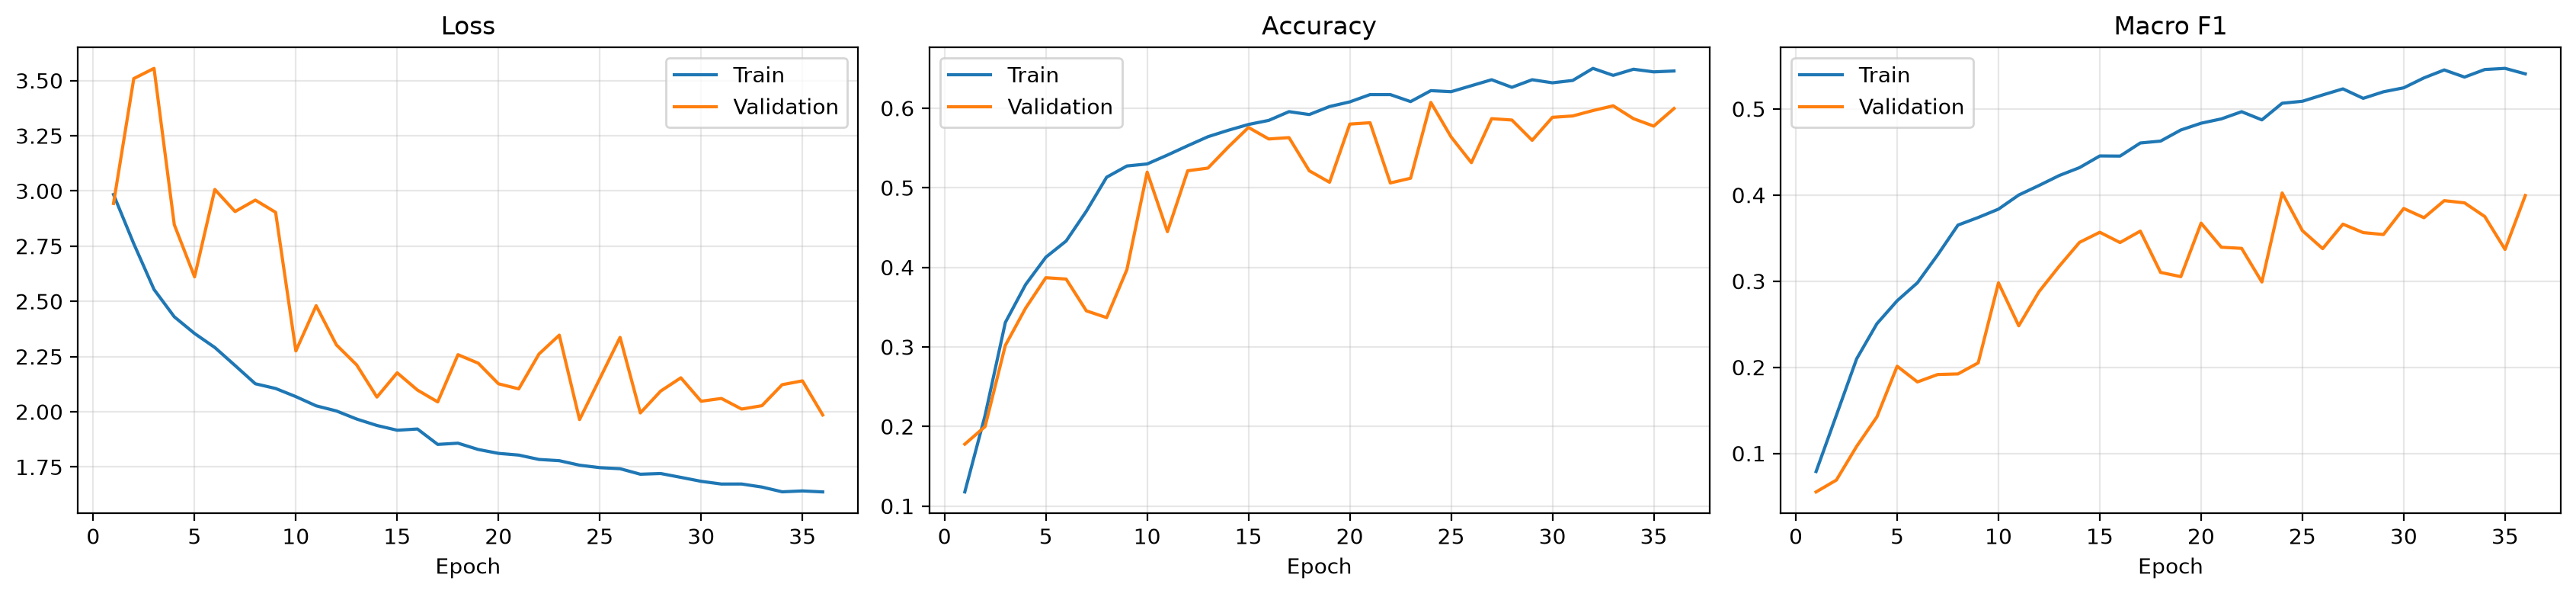
\includegraphics[width=\textwidth]{figures/training_curves_2d.png}
\caption{Pose 2D}
\end{subfigure}
\hfill
\begin{subfigure}[t]{0.49\textwidth}
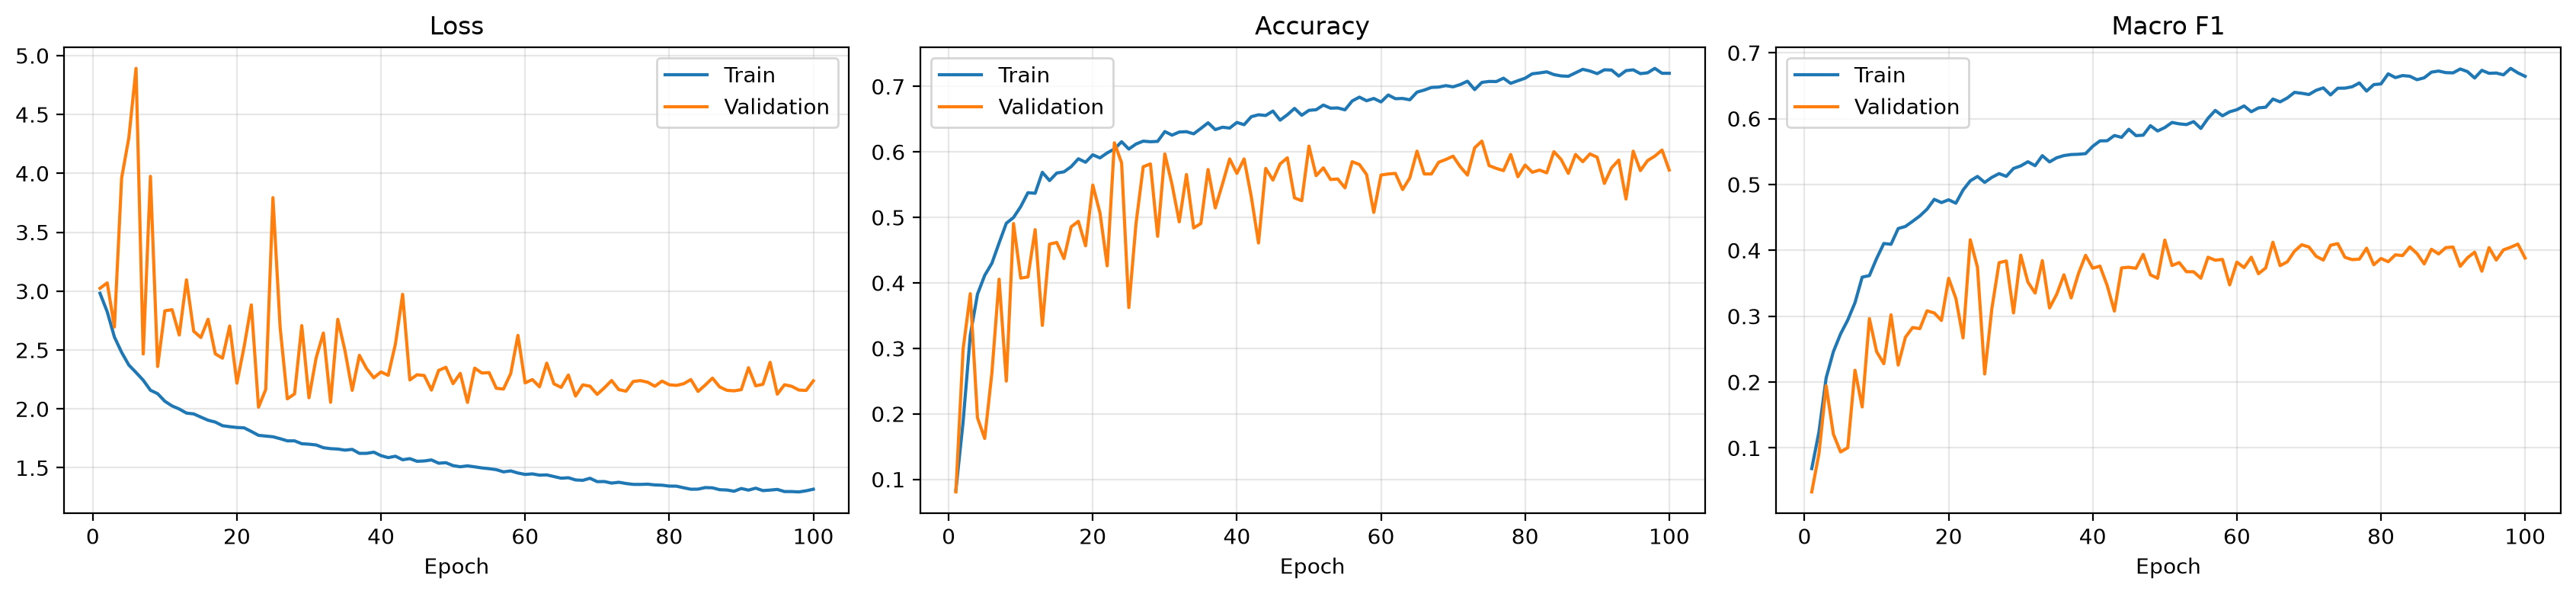
\includegraphics[width=\textwidth]{figures/training_curves_motionbert_3d.png}
\caption{Pose 3D MotionBERT}
\end{subfigure}
\caption{Đường cong huấn luyện của hai cấu hình}
\end{figure}

\begin{figure}[H]
\centering
\begin{subfigure}[t]{0.49\textwidth}
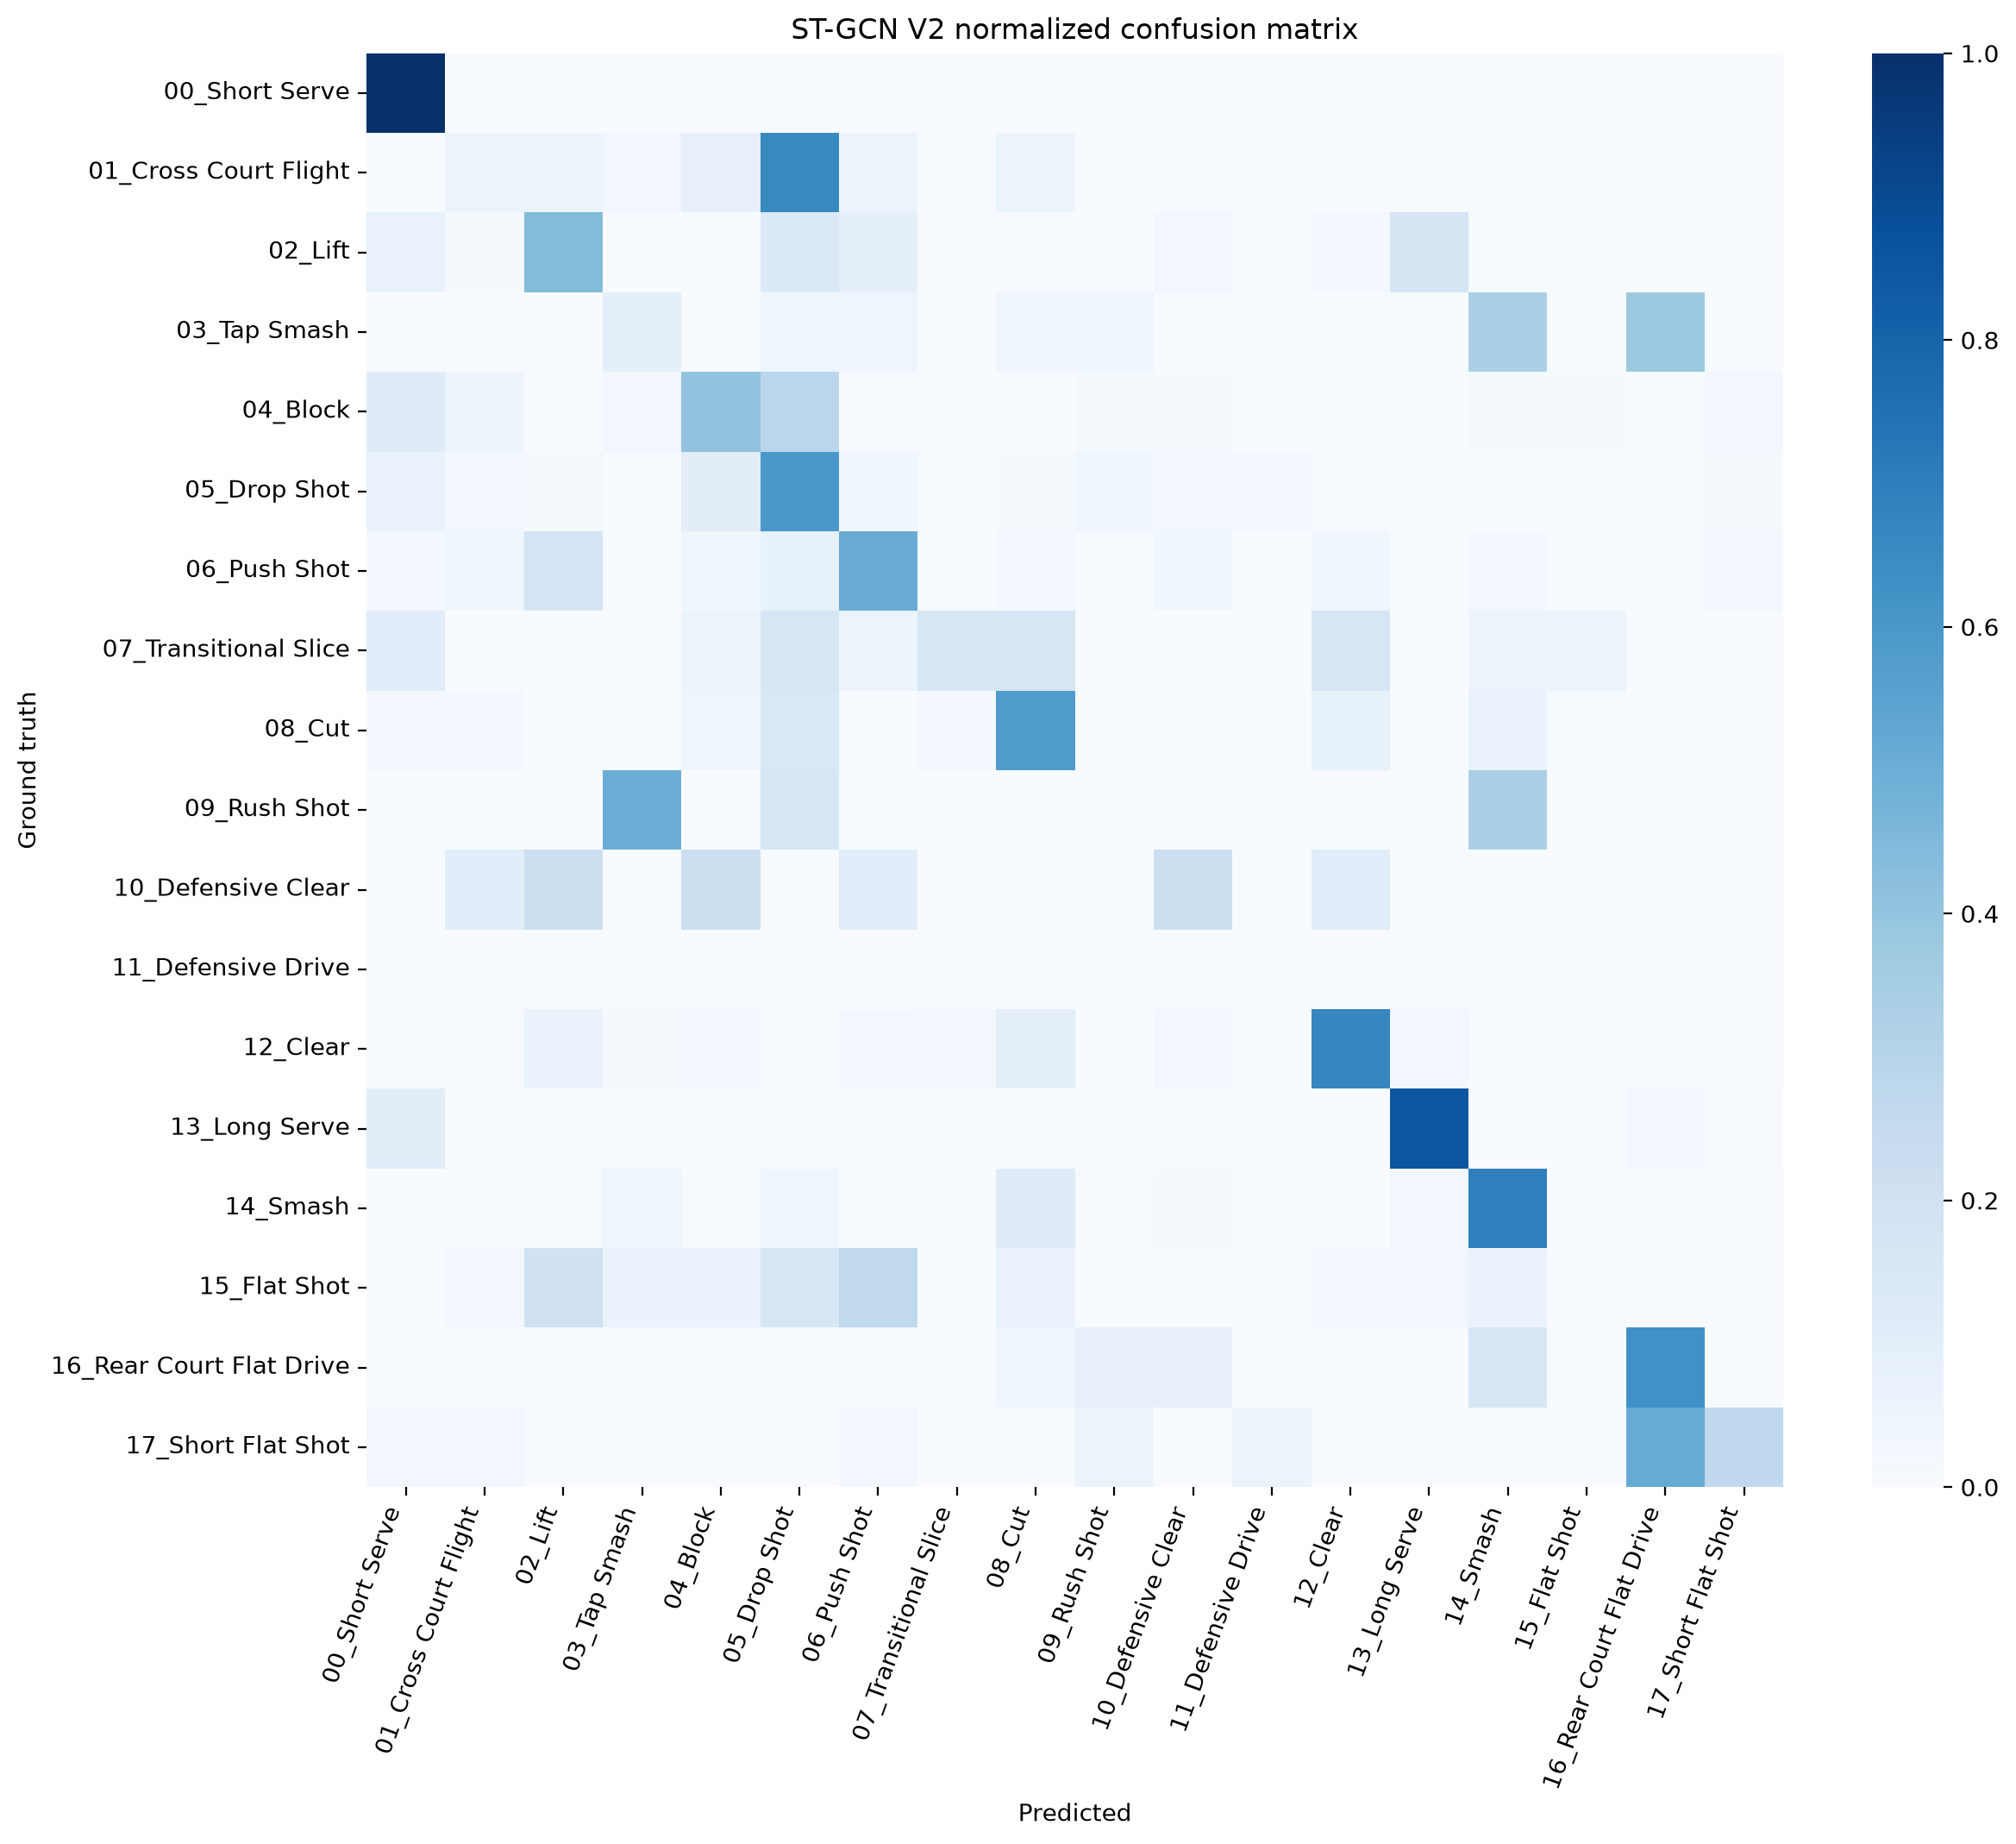
\includegraphics[width=\textwidth]{figures/confusion_matrix_2d.png}
\caption{Pose 2D}
\end{subfigure}
\hfill
\begin{subfigure}[t]{0.49\textwidth}
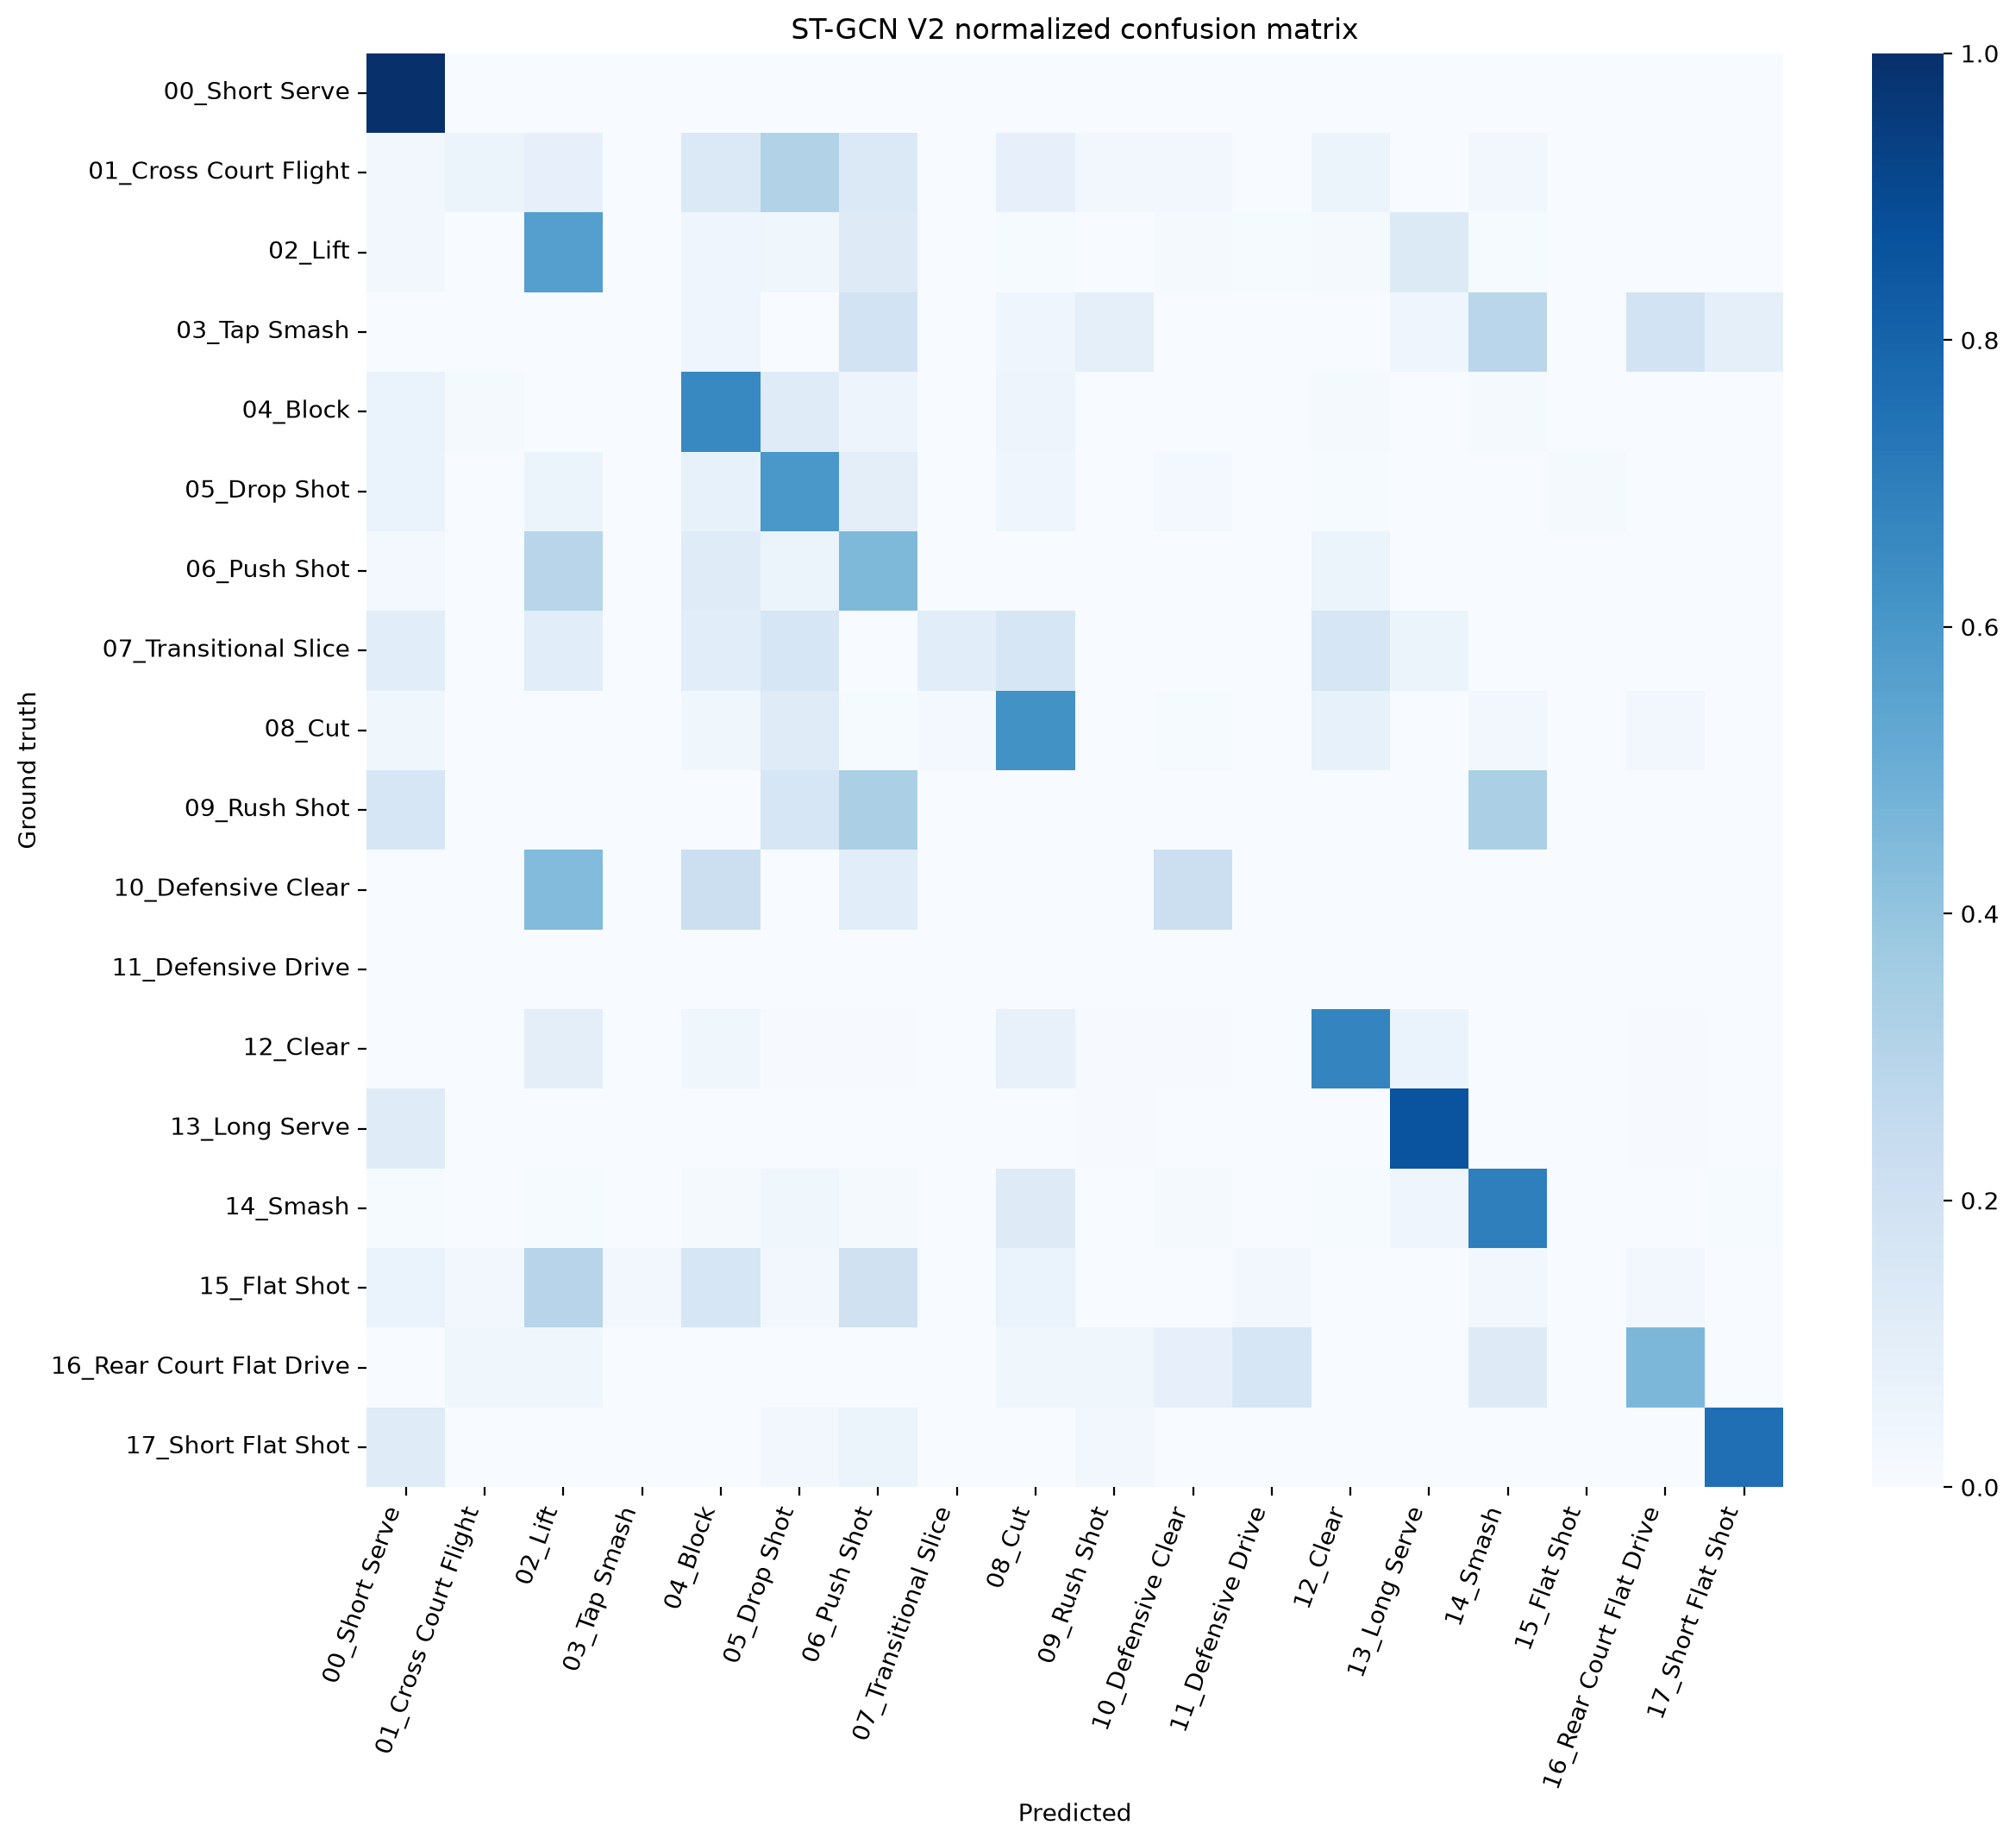
\includegraphics[width=\textwidth]{figures/confusion_matrix_motionbert_3d.png}
\caption{Pose 3D}
\end{subfigure}
\caption{Ma trận nhầm lẫn chuẩn hóa}
\end{figure}

\section{Kết quả theo lớp}

Với nhánh 3D, các lớp có F1 cao gồm Short Serve 0,841; Long Serve 0,828; Short Flat Shot 0,820; Smash 0,755 và Clear 0,743. Tap Smash, Rush Shot và Flat Shot có F1 bằng 0. Defensive Drive cũng có giá trị 0 nhưng không có mẫu test, nên không thể xem đây là đánh giá chất lượng thực tế. Các lớp yếu thường ít mẫu hoặc phụ thuộc vào góc vợt, thời điểm tiếp xúc và quỹ đạo cầu, là thông tin không có trong skeleton.

\section{Ablation trên pose 2D}

\begin{table}[H]
\centering
\caption{Các thí nghiệm ablation đã hoàn thành}
\begin{tabular}{lrrrr}
\toprule
\textbf{Cấu hình} & \textbf{Kênh} & \textbf{Người} &
\textbf{Test Acc.} & \textbf{Macro F1}\\
\midrule
Joint baseline & 5 & 2 & 54,15\% & 0,3771\\
Joint + position & 8 & 2 & 57,54\% & \textbf{0,4076}\\
Joint + hitter heuristic & 5 & 1 & \textbf{58,14\%} & 0,3653\\
Joint + bone & 9 & 2 & 50,59\% & 0,3240\\
\bottomrule
\end{tabular}
\end{table}

Position cải thiện Macro F1 tốt nhất. Hitter heuristic tăng accuracy nhưng giảm Macro F1. Bone stream hiện làm giảm cả hai chỉ số, do đó cần kiểm tra lại cách chuẩn hóa và fusion. Bộ ablation dùng một suite huấn luyện riêng nên không thay thế trực tiếp kết quả ST-GCN V2 chính.


\chapter{TIẾN ĐỘ TRIỂN KHAI VÀ KHẢ NĂNG TÁI LẬP}

\begin{table}[H]
\centering
\caption{Trạng thái các hạng mục}
\begin{tabularx}{\textwidth}{p{4.2cm}p{2.8cm}Y}
\toprule
\textbf{Hạng mục} & \textbf{Trạng thái} & \textbf{Kết quả}\\
\midrule
Audit và manifest & \done & 7.821 clip, 18 lớp\\
Chia dữ liệu theo phiên & \done & 56/12/12 phiên, không trộn phiên\\
YOLO26 pose 2D & \done & 7.818 clip thành công\\
ST-GCN V2 2D & \done & Accuracy 60,17\%, Macro F1 0,3882\\
Ablation 2D & \doing & Đã hoàn thành 4 cấu hình\\
MotionBERT pose 3D & \done & COCO-17 sang H36M-17, có resume\\
ST-GCN V2 3D & \done & Accuracy 63,90\%, Macro F1 0,4209\\
Tổ chức lại repository & \done & src, scripts, experiments, notebooks, tests\\
Đánh giá nhiều seed & \doing & Hiện mới có seed 42\\
Court, vợt và shuttle & \doing & Chưa đưa vào mô hình chính\\
\bottomrule
\end{tabularx}
\end{table}

\section{Tổ chức mã nguồn}

Kho mã hiện gồm:
\begin{itemize}
\item \code{src/badminton_stroke/}: dataset, graph, ST-GCN và đường dẫn dùng lại;
\item \code{scripts/}: tiền xử lý, YOLO pose và MotionBERT extraction;
\item \code{experiments/}: huấn luyện 2D, 3D và ablation;
\item \code{notebooks/}: khám phá, trực quan hóa và cấu hình workflow;
\item \code{processed/}: manifest, pose, confidence và kết quả;
\item \code{experiments/runs/}: đầu ra cho các lần chạy mới;
\item \code{tests/}: smoke test cho cấu trúc và forward pass.
\end{itemize}

MotionBERT được quản lý trong \code{third_party/MotionBERT}. Notebook có thể xuất thành script bằng \code{tools/export_notebooks.py}.

\section{Kiểm thử}

Năm kiểm thử hiện có đều vượt qua:
\begin{enumerate}
\item notebook và script xuất ra đồng bộ;
\item script import được mà không tự chạy pipeline;
\item tùy chọn \code{--help} hoạt động ngoài repository;
\item mọi code cell trong notebook biên dịch được;
\item ST-GCN forward được với cả 5 kênh COCO và 7 kênh H36M; logits hữu hạn và tổng attention của hai người bằng 1.
\end{enumerate}

\chapter{HẠN CHẾ VÀ KẾ HOẠCH TIẾP THEO}

\section{Hạn chế}

\begin{enumerate}
\item \textbf{Mất cân bằng lớp:} số mẫu train dao động từ 71 đến 680.
\item \textbf{Thiếu lớp trong test:} Defensive Drive không có mẫu test.
\item \textbf{Định danh người chưa liên tục:} quy tắc Top/Bottom được áp dụng độc lập từng frame, chưa có tracking.
\item \textbf{Người thứ hai thường vắng mặt:} slot Top chỉ hợp lệ trung bình 5,08\%.
\item \textbf{Chiều sâu là ước lượng:} MotionBERT có thể chịu domain shift và $z$ không phải khoảng cách vật lý.
\item \textbf{Thiếu vật thể tương tác:} skeleton không chứa vợt, shuttlecock và vị trí thật trên sân.
\item \textbf{Đánh giá mới dùng một seed:} chưa có trung bình và độ lệch chuẩn.
\item \textbf{Pipeline chưa end-to-end:} lỗi pose truyền sang classifier nhưng YOLO và MotionBERT chưa fine-tune theo loss phân loại.
\end{enumerate}

\section{Kế hoạch ưu tiên}

\begin{enumerate}
\item Chạy 2D và 3D với cùng lịch 100 epoch cho ít nhất ba seed.
\item Thiết kế group split có ràng buộc để mọi lớp có mẫu validation và test.
\item Đối chiếu trường \code{player} với slot người và bổ sung tracking hoặc hitter có giám sát.
\item Thực hiện ablation 3D riêng cho $z$, motion, confidence và person attention.
\item Bổ sung vị trí người trên sân bằng court homography.
\item Trích xuất shuttlecock và đặc trưng vợt rồi fusion với skeleton.
\item So sánh với 2s-AGCN, ST-GCN++ hoặc GCN--Transformer.
\item Xây dựng inference cho video mới và hiển thị xác suất theo thời gian.
\end{enumerate}

\section{Kết luận tiến độ}

Dự án đã hoàn thành pipeline từ video đến nhãn kỹ thuật, gồm kiểm tra dữ liệu, pose 2D, pose 3D, chuẩn hóa chuỗi, graph model và đánh giá. Nhánh MotionBERT 3D cải thiện kết quả lên accuracy 63,90\% và Macro F1 0,4209. Giai đoạn tiếp theo tập trung vào độ tin cậy của đánh giá, xử lý lớp hiếm, định danh người đánh và bổ sung court, vợt cùng shuttlecock.

\begin{thebibliography}{99}
\bibitem{videobadminton}
Q. Li, T.-C. Chiu, H.-W. Huang, M.-T. Sun, and W.-S. Ku,
"Benchmarking Badminton Action Recognition with a New Fine-Grained Dataset,"
\textit{arXiv preprint arXiv:2403.12385}, 2024.

\bibitem{stgcn}
S. Yan, Y. Xiong, and D. Lin,
"Spatial Temporal Graph Convolutional Networks for Skeleton-Based Action Recognition,"
\textit{Proceedings of the AAAI Conference on Artificial Intelligence},
vol. 32, no. 1, 2018.

\bibitem{motionbert}
W. Zhu et al.,
"MotionBERT: A Unified Perspective on Learning Human Motion Representations,"
\textit{Proceedings of the IEEE/CVF International Conference on Computer Vision},
2023.

\bibitem{ultralytics}
Ultralytics, "Pose Estimation with Ultralytics YOLO,"
\url{https://docs.ultralytics.com/tasks/pose},
truy cập tháng 11 năm 2026.
\end{thebibliography}

\appendix
\chapter{TỆP VÀ LỆNH TÁI LẬP}

\section{Thứ tự chạy}
\begin{verbatim}
uv sync --frozen
source .venv/bin/activate
python scripts/preprocess_data.py --non-interactive
python scripts/extract_yolo_pose.py --non-interactive
python scripts/extract_motionbert_3d.py --non-interactive
python experiments/train_stgcn_motionbert.py --non-interactive
\end{verbatim}

\section{Kiểm tra mã nguồn}
\begin{verbatim}
python tools/export_notebooks.py --check
python -m unittest discover -s tests -v
\end{verbatim}

\section{Thư mục kết quả}
\begin{verbatim}
processed/
|-- manifests/
|-- joints_npy_yolo26s_pose/
|-- scores_npy_yolo26s_pose/
|-- joints_3d_motionbert/
|-- scores_h36m_motionbert/
|-- stgcn_v2/
|-- stgcn_ablation/
+-- stgcn_v2_yolo26_motionbert/
\end{verbatim}

\end{document}

